%%%%%%%%%%%%%%%%%%%%%%%%%%%%%%%%%%%%%%%%%%%%%%%%%%%%%%%%%%%%%%%%%%
%%%%%%%% ICML 2015 EXAMPLE LATEX SUBMISSION FILE %%%%%%%%%%%%%%%%%
%%%%%%%%%%%%%%%%%%%%%%%%%%%%%%%%%%%%%%%%%%%%%%%%%%%%%%%%%%%%%%%%%%

% Use the following line _only_ if you're still using LaTeX 2.09.
%\documentstyle[icml2015,epsf,natbib]{article}
% If you rely on Latex2e packages, like most moden people use this:
\documentclass{article}
\newcommand\tab[1][1cm]{\hspace*{#1}}

% use Times
\usepackage{times}
% For figures
\usepackage{graphicx} % more modern
%\usepackage{epsfig} % less modern
\usepackage{subfigure} 

% For citations
\usepackage{natbib}
\bibliographystyle{unsrtnat}

% For algorithms
\usepackage{algorithm}
\usepackage{algorithmic}

% As of 2011, we use the hyperref package to produce hyperlinks in the
% resulting PDF.  If this breaks your system, please commend out the
% following usepackage line and replace \usepackage{icml2015} with
% \usepackage[nohyperref]{icml2015} above.
\usepackage{hyperref}

% Packages hyperref and algorithmic misbehave sometimes.  We can fix
% this with the following command.
\newcommand{\theHalgorithm}{\arabic{algorithm}}

% Employ the following version of the ``usepackage'' statement for
% submitting the draft version of the paper for review.  This will set
% the note in the first column to ``Under review.  Do not distribute.''
% \usepackage{icml2015} 

% Employ this version of the ``usepackage'' statement after the paper has
% been accepted, when creating the final version.  This will set the
% note in the first column to ``Proceedings of the...''
\usepackage[accepted]{icml2015}

% The \icmltitle you define below is probably too long as a header.
% Therefore, a short form for the running title is supplied here:
\icmltitlerunning{Yelp Challenge: Rating Prediction}

\begin{document} 

\twocolumn[
\icmltitle{Yelp Challenge: Rating Prediction}

\icmlauthor{Yuanjian Lai}{lai.yua@husky.neu.edu}
\icmladdress{Northeastern University,
 360 Huntington Ave, Boston, MA 02110}
\icmlauthor{Zhikai Ding}{ding.zhika@husky.neu.edu}
\icmladdress{Northeastern University,
           360 Huntington Ave, Boston, MA 02110}

% You may provide any keywords that you 
% find helpful for describing your paper; these are used to populate 
% the "keywords" metadata in the PDF but will not be shown in the document
\icmlkeywords{boring formatting information, machine learning, ICML}

\vskip 0.3in
]

\section{Introduction}

Yelp Challenge provides data scientists with a great source for machine learning and data mining experiments. In this project we investigate the factors that decides a business's rating. This knowledge is especially valuable to business owners, who can use the knowledge to predict the performance of their businesses so as to make important decision and make their business successful. To make better concentration, we limit our experiments on restaurant business.  After preprocessing data to handle missing values and mapping raw features into numeric features, we use clustering algorithm to generate features like location cluster and cluster size feature (from longitude and latitude). After that we use feature selection technology to reduce the data dimensionality and to remove the noise features. In the evaluation section, we evaluate our result against random guest result, a baseline result, by both accuracy and RMSE. We use grid-test to select the optimal parameters for different models. And cross-validation is used to computed the accuracy for those models.  


\section{Data Preprocessing}

Firstly a naive data processing scripts is used to parse the business data and count the number of record to get a general view of the data set. we have for different business. Below is the figures of the top frequent categories among the whole data set (77445 businesses of 962 categories):
\begin{itemize}
\item Restaurants: 25071
\item Shopping: 11233
\item Food: 9250
\item Beauty \& Spas: 6583
\item Health \& Medical: 5121
\item Night life:5088
\end{itemize}

Furthermore, if we narrow the scope to restaurants businesses, new figures come out, below are the top frequent ones among 296 categories for the 25071 businesses related to Restaurants:
\begin{itemize}
\item Fast food: 2851
\item Pizza: 2657
\item Night life: 2533
\item Mexican:2515
\item Bars: 2423
\item American (Traditional): 2416
\item Sandwiches: 2364
\item Food: 2101
\end{itemize}

We can notice that the categories have many overlaps: a pizza restaurant is very likely also marked as fast food restaurant, some bar-like restaurants may be categorized as Night life place as well. Hence in the model selecting part, we should take this into account.

There is another tricky part of the data set. For the business, we get most of the information from its attributes. And in most of the machine learning regression models, we would like to map those features into numeric ones. However, some attributes are missing for some data record. 
One thing we can do is to simply filter those records out. Only picks those record that has the necessary features. But this could significantly shrink our the size of our dataset. Additionally, to do this we should firstly manually define that which features among those features are relatively more important. This can incur more  inaccuracy as well since this is not data-driven decision and we are not a professional/expert in this domain.
Otherwise, we can set the missing feature to a default value. This might undermine the performance of certain models too, but basically this is the best we can do compared to other options.

In order to map the features to a numeric value, we write scripts to analyze each feature in the data set, and count how many records have the values. The analysis report is following (Only consider those records that have Price Range):
\begin{itemize}
\item Review count (share by all business)
\item Accept Insurance: False:2, NA: 23402, (ignored)
\item Drive-Thru: False: 1798, True: 1475, N/A: 20131, N/A regarded False
\item Alcohol: none:9391,beer and wine:3090,full bar:7802, N/A:3121
\item Open 24 Hours: False: 222, NA: 23164, True: 18 (ignored)
\item Noise Level:  very loud:561, average:12550, loud:1482, quiet:4290, N/A
\item Music: dj: 1859, background music: 854, jukebox: 1271, live: 1257, video: 1165, karaoke: 866 (Enumeration) (ignored)
\item Attire: formal:56,dressy:769,casual:21627,N/A:592
\item Ambience: romantic: 18984, intimate: 18984, classy: 18984, hipster: 18866, divey: 18425, touristy: 18984, trendy: 18984, upscale: 18879, casual: 18984 (Enumeration)
\item Good for Kids: False: 3847, True: 18367, NA: 1190
\item Price Range: 1: 10498, 2: 11240, 3: 1378, 4: 288
\item BYOB: False: 786, NA: 22576, True: 42
\item Caters: False: 7832, True: 7444, NA: 8128
\item Delivery: False: 17536, True: 4224, NA: 1644
\item Dogs Allowed: False: 1822, True: 543, N/A: 21039 (ignored)
\item Coat Check: False: 2097, True: 158, N/A: 21149 (ignored)
\item Smoking:  yes: 295, outdoor: 1181, N/A: 20881, no: 1047
\item Accepts Credit Cards: False: 888, True: 21925, N/A: 591
\item BYOB/Corkage: yes corkage: 142, N/A: 22118, yesfree: 464, no: 680 (ignored)
\item Take-out: False: 2023, True: 20234, N/A: 1147
\item Ages Allowed: 19plus: 1, 21plus: 16, N/A: 23377, allages: 7, 18plus: 3 (ignored)
\item Corkage: False: 490, True: 128, N/A: 22786 (ignored)
\item By Appointment Only: False: 22, True: 2, N/A: 23380 (ignored)
\item Happy Hour: False: 395, True: 1975, N/A: 21034 (ignored)
\item Wheelchair Accessible: False: 1057, True: 10393, N/A: 11954 (ignored)
\item Outdoor Seating: False: 12531, True: 9371, N/A: 1502
\item Takes Reservations: False: 14001, True: 7821, N/A: 1582
\item Waiter Service: False: 7670, True: 12802, N/A: 2932
\item Wi-Fi: paid: 155, N/A: 6564, free: 6396, no: 10289
\item Dietary Restrictions:dairy-free: 145, gluten-free: 145, vegan: 145, kosher: 145, halal: 145, soy-free: 145, vegetarian: 145 (ignored)
\item Good For Dancing: False: 1979, True: 331, N/A: 21094 (ignored)
\item Order at Counter: False: 137, True: 228, N/A: 23039 (ignored)
\item Good For: dessert: 21152, latenight: 21205, lunch: 21205, dinner: 21205, brunch: 21154, breakfast: 21213 (Enumeration)
\item Parking: garage: 20496, street: 20494, validated: 20306, lot: 20494, valet: 20494 (Enumeration)
\item Has TV: False: 10105, True: 9920, N/A: 3379
\item Good For Groups: False: 2488, True: 19969, N/A: 947
\end{itemize}

As you can see, among those features, there are some are held by very few records (such as Accept Insurance, Open 24 Hours). Since we can not guess a ad-hoc value for the commonly missing features, we just simply ignore them in this experiments. (marked as ignored)

There are also some features that are not boolean nor numeric, which are more like a enumeration value (marked as enumeration). For these features, we map each enumeration to a feature.
For example: the Parking has 5 possible value, we map each value into a single features
and for Attire, we simply map each enumeration to a numeric value

\subsection{Generated Features}
There are some features that cannot be directly used, such as longitude and latitude. We use K-means to cluster those features. By doing this, two new features has been added to the data, the cluster label and cluster size.
\section{Feature Selection}
There are three classes of feature selections, they are filtering method, wrapper method and embedded method. In this project, we decided to use RFE (filtering) to select a subset of features to reduce the data dimensionality and to enhance the accuracy. By RFE, a side-product is that we can know which features are relatively more important than others. This output is also valuable to the business owner.
Recursive Feature Elimination(RFE) is a popular and widely used feature selection method, which means recursively fitting a model use different number of features. After which it ranks the features by their importance and select the optimal number of features by the accuracy.
In this project we use Multinomial Logisitc Regresion as the model for feature selection. The accuracy graph is shown below.
\graphicspath{ {images/} }
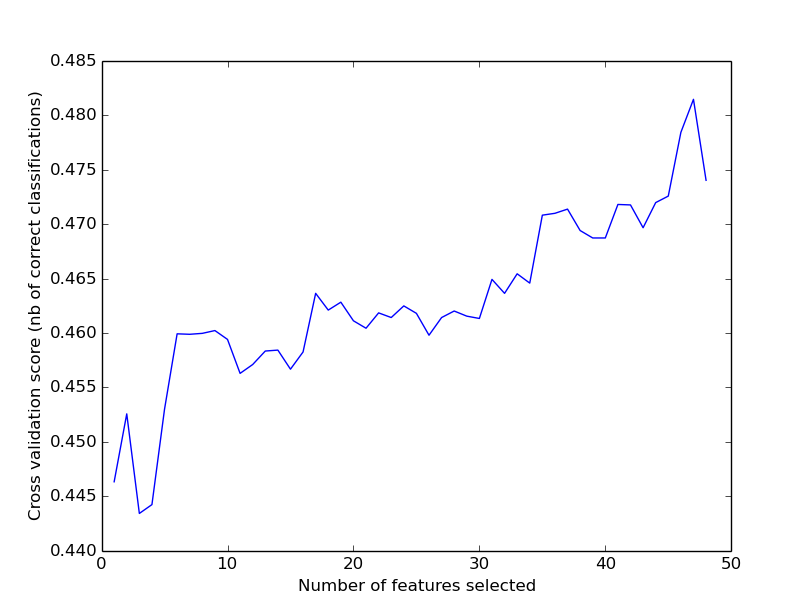
\includegraphics[scale=0.4]{RFEMLR}
The top 3 most import features are Delivery, Drive-Thru and Take-out
%\section{Models}
%\subsection{Multinomial Logistic Regression}
%\subsection{Decision Tree}
%\subsection{Random Forest}
%\subsection{Multinomial Naive Bayes}
%\subsection{SVM(SVC)}


\section{Evaluation And Results}

\subsection{Evaluation Function}
Since rating has numeric meaning, apart from accuracy, we also apply RMSE to evaluate models. The rating scale from 0 to 5 and the RMSE implies the average difference between the predicted rating and the true rating.
\subsection{Random Measure}
If we randomly guess the value, the accuracy should be 1/5. which is approximately 20\%.

\subsection{Baseline Measure}
Because we are building a regression model, we used the central tendency measure as our baseline. That is, to calculate the median, mode and mean of our prediction of the rating of test data set, and then compare them with the actual ratings of the test data set.
We compute the mean and the distribution of the dataset's rating, the mean is 3.24, and the distribution is below:
\begin{center}
\begin{tabular}{| l | l | l | l |}
    \hline
Rating & Number of Records & Percentage \\ \hline
1 &431 &0.018  \\ \hline
2 &3189 &0.136  \\ \hline
3 &10446 &0.446  \\ \hline
4 & 8927 &0.381  \\ \hline
5 &411& 0.017  \\ \hline
\end{tabular}
\end{center}

We can observe that the mode of the rating is 3, and baseline of accuracy should be 44.6\%, the baseline of RMSE is 0.81.
\section{Conclusion}
We fit 5 models, Multinomial Logistic Regression(MLR), Decision Tree, Random Forest, Multinomial Naive Bayes(MNB) and SVM. The accuracy of the results are from 26\% to 47\%, among those models, Random Forest, SVM and Multinomial Logistic Regression (MLR) have the same accuracy 47\%. The RMSE is from 1.58 to 0.81, among those models, the SVM performs best (with least RMSE 0.81)
\begin{center}
    \begin{tabular}{| l | l | l | l |}
    \hline
    Model & Parameters & Accuracy (\%) & RMSE \\ \hline
	MLR &  C=4 & 47 (+/- 4) & 0.86\\ \hline
    Decision Tree & & 40 (+/- 2) &1.03 \\ \hline
    Random Forest & ntrees=10& 43 (+/- 3) & 0.96\\ \hline
    MNB & alpha=1& 26 (+/- 4)&1.58 \\ \hline
	SVM & tol=0.001 C=0.001& 47 (+/- 3) & 0.81\\ \hline
    \end{tabular}
\end{center}

\end{document} 



\bibliography{example_paper}

\end{document} 


% This document was modified from the file originally made available by
% Pat Langley and Andrea Danyluk for ICML-2K. This version was
% created by Lise Getoor and Tobias Scheffer, it was slightly modified  
% from the 2010 version by Thorsten Joachims & Johannes Fuernkranz, 
% slightly modified from the 2009 version by Kiri Wagstaff and 
% Sam Roweis's 2008 version, which is slightly modified from 
% Prasad Tadepalli's 2007 version which is a lightly 
% changed version of the previous year's version by Andrew Moore, 
% which was in turn edited from those of Kristian Kersting and 
% Codrina Lauth. Alex Smola contributed to the algorithmic style files.  
